\documentclass[11pt,a4paper]{book}
\usepackage[english]{babel}
\usepackage{amsmath}
\usepackage{amsthm}
\usepackage{amsfonts}
\usepackage{amssymb}
\usepackage{graphicx}
\usepackage{geometry}
\usepackage[percent]{overpic}
\usepackage{tikz}
\usepackage[titletoc]{appendix}
\usepackage[round]{natbib}


%\usepackage[usenames,dvipsnames,svgnames,table]{xcolor}
\definecolor{kuleuven}{RGB}{29,141,176}
\definecolor{kuleuven1}{RGB}{82,189,236}


\newcommand{\nocontentsline}[3]{}
\newcommand{\tocless}[2]{\bgroup\let\addcontentsline=\nocontentsline#1{#2}\egroup}

\newcommand\numberthis{\addtocounter{equation}{1}\tag{\theequation}}



\allowdisplaybreaks




\makeindex

\begin{document}
%Start
\frontmatter
\newgeometry{textwidth=540pt,textheight=780pt,top=20pt,left=20pt,right=20pt}
\begin{titlepage}

\begin{figure}[t]{%
      \begin{overpic}[width=1\textwidth]{../LaTeX/Layout/Picture1.png}
         \put(46,4){\color{white}\large{\textbf{FACULTY OF ECONOMICS AND BUSINESS}}}
      \end{overpic}
    }
\end{figure}

\vspace*{4.5cm}
{\color{kuleuven1}{\Huge  A survey on the impact of customer service chatbots on e-commerce}}

\vspace*{0.5cm}
{\Large Type your subtitle here}

\begin{figure}[b]
  %\centering
   \begin{minipage}[c]{0.4\textwidth}  {%
      \begin{overpic}[width=0.9\textwidth]{../LaTeX/Layout/Picture2.png}
         \put(70,45){\begin{minipage}[c]{1.80\textwidth}
\begin{flushright}

{\Large Rob De Putter, Mout Pessemier, Laurens Van Keymolen} \linebreak
{r08, r0837708, r} \linebreak

\textbf{{\large Thesis submitted to obtain \linebreak
the degree of}} \linebreak

%!!!IMPORTANT!!!:
%indicate the appropriate title of your master and major. Check the website https://feb.kuleuven.be/studentenportaal/contact/masterproef-leuven
{\large Informatiemanagement}\linebreak
{\large ???}\linebreak
\linebreak
\textbf{{\large Promoter:}}   Prof.\ Dr.\ Jan Vanthienen \linebreak
\textbf{{\large Co-promoter:}} Prof.\ Dr.\ ... \linebreak
\textbf{{\large Tutor:}} Prof.\ Dr.\ ... \linebreak

%\linebreak

\textbf{{\large Academic year:}} {\large 2021-2022}
\linebreak
\end{flushright}
  \end{minipage}}
      \end{overpic}
    }
  \end{minipage}


\begin{picture}(540,0.2)
\put(0,0){\colorbox{kuleuven1}{\makebox(540,0.2){}}}
\end{picture}
\end{figure}

\end{titlepage}
%%%%%%%%%%%%%%%%%%%%%%%%%%%%%%%%%%%%%%%%%%%%%%%%%%%%%%%%%%%%%%%%%%%%%%%%%%%%%%%%%%%%%%%%%%%%%%%%%%%% 

\restoregeometry
\setcounter{equation}{1}

\pagestyle{empty}
\tableofcontents



%Abstract
\chapter*{Abstract\hfill} \addcontentsline{toc}{chapter}{Abstract}
\label{ch:abstract}
\begin{flushright}
	Leuven, May, 2022.
\end{flushright}
%%%%%%%%%%%%%%%%%%%%%%%%%%%%%%%%%%%%%%%%%%%%%%%%%%%%%%%%%%%%%%%%%%%%%%%%%%%%%%%%%%%%%%%%%%%%%%%%%%%%%%%%%
\acrfull{ai} has grown ingrained in the \acrshort{it} sector, and technology is increasingly incorporated into our daily lives. Businesses are aware of this switch and are trying to use \acrshort{ai} to automate repetitive and ordinary work, which results in a more efficient and productive way of working. Customer service chatbots are an example of this. These "robots" are ideally capable of largely taking over the customer service from human agents. It is critical that these chatbots continue to produce high-quality work in order to improve customer experience and satisfaction, as this has a significant impact on customer trust and brand reputation.\\
\break
The goal of this research is to determine the impact of chatbots on companies' current and future strategies, as well as what customers expect from such a chatbot. The research is applied within the scope of the Belgian and Dutch telecom industries. Interviews with telecom companies such as Proximus, Telenet, T-Mobile, and KPN were done as part of this research, as well as a survey to get customer insights/expectations on these chatbots and what is important to them.\\
\break
The results show that in the future, telecom providers want to optimise their chatbots through data analysis, with sentiment analysis as the most common approach. From the importance study, it can be concluded that the chatbot should be easy to use and available 24/7.

%Eigenlijke tekst
\mainmatter
\pagestyle{headings}

\chapter{Introduction}
Example citation: \cite{von2007theory}


\begin{figure}
	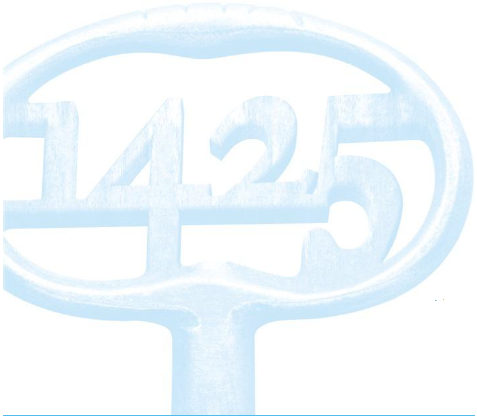
\includegraphics[width=0.2\textwidth]{../LaTeX/Figures/Picture2.png}
	\caption{Example figure}
\end{figure}





%Bijlagen
\begin{appendices}
	\chapter{Business Interviews}
	\label{ch:appendices}
	The write-out of these interview are a streamlined version. It's not a literal transcription to increase readability and because most of these interview had to be translated from Dutch to English.
	
	\section{Interview with Proximus}
	\label{in:Proximus}
	\subsection{The current state of the customer service chatbot.}
	\subsubsection{For what purposes is the conversational agent mainly used? Is it for \acrshort{faq}, to assist the help desk, deal with complaints, helping with sales or other functionalities?}
	At Proximus it was designed for support questions for residential people. That means you, me, your family, …. It’s not developed for small businesses. The goal is to help the small customers who can’t find an answer on the \acrshort{faq} pages or help centre. It also offers a new way to get requests solved in a new, innovative, fast and personalised way. That is really the first goal. Then we saw that people were also using this to ask questions about specific products or specific subscriptions. So, at some point we also had to include more sales topics. Today we really have support and sales. Our goal is to go towards the next best action, promotion, etc. But that is for the future. It’s mainly used for support.
	
	\subsubsection{And complaints?}
	People come to the bot and complain but we don’t want to offer an automatic response “okay then you go to this page and do that”. When they complain, we capture the complaint and send it to an agent. An agent is a live person.
	
	\subsubsection{What about the platform with which the customers can interact with the chatbot? Is it solely on the website or can you use it via social media, the Proximus platform or any other media?}
	We have 3 channels today. Our website, the app and Facebook Messenger. The goal is to have the chatbot at some point available through the telephone.
	
	\subsubsection{As a stand-alone application or?}
	Mainly to replace the call centers. So today, if you for example don’t have internet, you call a live agent. The goal is in the future to have intent detection directly there and have a more conversational experience rather than “press 1” or “press 2”.
	
	\subsubsection{In which languages can the chatbot be used? Dutch? French? English? Any others?}
	Dutch, French and English are available for all conversations. With our artificial intelligence, we can detect if you are talking in German or Italian and say “that’s not a language we are covering” and then propose English.
	
	\subsubsection{Why specifically these languages?}
	We live in Belgium, those are the most important languages. We also don’t have any German speaking colleagues for example, and we don’t want to Google Translate our bot. It’s also a legal requirement to have this.
	
	\subsubsection{Since Proximus is a Belgium based company, do you feel that there isn’t a need to support other languages?}
	It’s not that there is no need. It’s quite marginal. We do have expat coming to Belgium. They speak English. Our bot is really big so if we want to translate everything in another language, it means rebuilding everything and we just decided to tackle the long tale, not the short tale.
	
	\subsubsection{Do you have a rough estimate of what the \% is of different age groups that interact with the chatbot?}
	We don’t know that today. It’s not that I don’t want to provide this to you, it’s that we don’t know. I can say from manually checking conversations that is it widely spread. We have customers that are super easy with technology and that know how to use a bot. When the bot says, “can you please repeat your sentence”, that they try in an easy way to rephrase their question. We have people that don’t click on buttons and keep saying that it isn’t working. We have all of the different kind of people.
	
	\subsubsection{Do you have any idea as to why there is such a big spread?}
	Because our clients are a large group. Proximus has a position on the market to fill student needs, family needs, individual needs. We have Scarlet and Mobile Vikings. We have subscription packs for different types of families. Packs for adults, packs for students? We have pre-paid cards. It’s super broad. Our scope handles more than 450 questions a day because there are so many different questions that you can ask. It’s super broad.
	
	\subsubsection{That directly brings me to my next question. Because there are a lot of different questions, which types of questions can it answer? Only yes/no question or also open questions, very specific questions? Do we have to ask very specific questions, or can we be more vague?}
	Yes, and yes. If the question is vague, we can detect that we are missing some information and tell the customer: “okay we understand you have a question about x, here is what I can do” and then redirect. But if you say something super specific like “I forgot my pin code”, we can also provide help. Both approaches are used to not miss a conversation.
	
	\subsection{The benefits that the chatbot brings to Proximus.}
	\subsubsection{What type of services does the chatbot provide? Can it for example extend a membership or replace a pin code as you said. Or is it mainly used to redirect to the correct pages and not per se execute a task.}
	I get your question. What you must know is, once we want to be transactional, so get your pin code and not give a general answer, it needs a lot of development, and it has a impact on a lot of different teams. There is an ambition to have more transactional conversations, it’s just not feasible in the short term. So, what we can do is retrieve your pin code based on your phone number and client number, we can retrieve your bill balance to know how much you still have to pay. You can do promise of payment. It’s for people who pay later and promise to pay, we then have his promise of payment, and their service won’t be deactivated. You can ask for payment deferrals when you want to pay your bill one week later. That’s all what the bot will do in the backend as transactional conversations. We can verify the state of your subscriptions and services. I don’t know if you know but in telco, if you don’t pay your bill, you get lower speed for internet. So, when people complain about it, we can say “that’s because you didn’t pay your bill”. We can reset pin codes. You have a pin code for your phone, one for your tv. That’s something we can all reset in the backend. That’s our big bucket for now what we can do.\\
	Our strategy is of course to provide solutions, not instructions. With instructions I mean “for that task, you can go to this page where we have an explanation for you. This is your problem, here is your solution.”
	
	\subsubsection{Since you described the whole transactional conversation. Which conversation type right now is the most occurring? Transactional or informational?}
	There is less transactional conversation because we are covering more than 450 topics, we need to decide from a strategy point of view, what do we want to ‘transactionalise’, what is best for the customer depending on the channel. With a chat on the website, it is easier to say “for that you need to order that” via a webform because it was made for that interface. For some questions, we know that the website cannot help, that the \acrshort{faq} nor helpdesk can help, the self-service is not available, so we need an agent. Either we do a transaction or guide them to the best place to do it or we explain as best we can how to do it. That’s sometimes also the case.
	
	\subsubsection{My next question is about the customer service employees and their workload. As you said the chatbot will not be perfect and some questions have to be answered by agents. Do you have a rough estimate how much percent of questions a chatbot cannot answer?}
	That, I’m not sure I can really share. What I can share is that we decided that some topics we are not covering. So, that’s also part of how you design the chatbot. If you have a lot of questions about something that is not your scope, that we know we decide not to cover. The thing is, today as said, 450 questions is already a lot, but you can imagine to get there, there were a lot of analyses done. Of course, there is still a lot that we are not covering but that’s also because it doesn’t make sense to putting our focus on that.
	
	\subsubsection{What about the willingness of the customers? Today there is still a lot of pushback towards the usage of chatbots from the general masses. The feeling that they can’t help you or that they never will be able to replace a real human is real. How many of your customers are willing to use the chatbot?}
	It’s a difficult number to get because you need to ask the people “would you like to use the chatbot?” and then they would say this or that. From the analysis and benchmarking we’re doing, and from my personal story, I’m working with chatbots for over five years now, and I still ask another chatbot “Can I talk to a human”. At the end of the conversation, you can rate the conversation and sometimes you can leave open feedback. We see that people are super happy when the bot was super accurate with its response. Since it is transactional, the answer is personalised. Or when the bot is really fast. For example, with a small question, then the user got his answer very quickly. Or it is an easy step process. Say you want to do something and it’s only three steps, then the bot can say do this, this and this. Redirection to the right place, so we really help the customer so that they are really happy. Those customers will be eager to retry to use the bot.\\
	\break
	What really doesn’t work is when the bot doesn’t understand. So, an infinite loop with the bot saying: “sorry I don’t understand”. We try to be as human as possible, so we don’t repeat the phrase “sorry I don’t understand” twice but we vary. It depends on the state of mind of the person. If he’s in a nice state of mind, he will be patient and he will repeat his question. If he’s super angry because e.g., he didn’t pay his bills or he has a lot of trouble with paying his bills, he won’t have the patient. Also, here, the bot is not relevant to help.\\
	\break
	People that are patient and okay with technology they will use and reuse the bot. People that are not comfortable with technology or people who have a really big problem, and the bot doesn’t understand won’t reuse the bot. A bot is there to help easy and short questions. So, for everything that’s not in there, people won’t be eager to retry.
	
	\subsubsection{Since you said that people can leave rating after a certain conversation. Do you have an estimate whether they are mostly positive or negative ratings?}
	We have both. It’s either super positive or super negative but never in between. It’s human behaviour. If you are super happy you say ‘okay, that was great’. If you are super unhappy, you will take the time to say it. The thing is, the question is randomly triggered. It’s not triggered at the end of each conversation to have open feedback. That way we don’t want to overload our systems. So, you might fall on the person that would love to leave a comment but wasn’t offered the possibility.
	If the bot doesn’t understand, we will always take that feedback. If the user is super unhappy about Proximus in general, not only about the conversation, we also filter on that.
	
	\subsubsection{This perfectly bring us to the next question. I wanted to ask you if there are any negatives linked to the usage of a chatbot. For example, is there more user frustration right now or are there more complaints or is it the other way?}
	There were different steps. We first started with the live chat. So, when you were on the Proximus website you would directly have an agent. People were super happy because when they had a question, they almost immediately had an answer. Then we introduced the bot with \acrshort{nlp} that wasn’t great and super large. For example, when you said, “I want to cancel my Netflix account”, the bot understood: “Ah, okay, you have a question about Netflix. What do you want to do?” It was really not friendly. The difference between those 2 solutions was quite frustrating for the user. Today we have both super happy and super unhappy customers. In the super unhappy customer group, we have frustrated customers because the bot did not do well. That’s our fault. We also have unhappy customers because their internet is not working, they try to contact the bot and it doesn’t work and they feel like “I pay so much money for this and the service doesn’t work”. In the middle it’s difficult to say. But we also see, because now we are also experimenting with voice, that people are not yet ready to communicate with voice. It’s another interface. In the United States, they communicate with Siri and Alexa all the time but here, managing how to answer, what to answer, the length of the answer, … It’s really complicated so it will be even more frustration for the customer in the future.
	
	\subsubsection{Do you think that during the time where the bot wasn’t as fluent and as well put together as it is now the company a lot of customers? Was there a lot of customer churn because of the chatbot or do you think that having a bad chatbot did not impact the customer churn much at all?}
	To be honest, no, because today, unofficial number show that 10\% of interactions are done by the bot, 90\% are done via call. If out of the 10\% done by the bot, you have 50\% not happy about the bot then you need also to split between was it really the bot or Proximus in general etc. It’s difficult to say.\\
	\break
	You cannot push people away with the bot. Maybe a small percentage but they are mostly already leaving and use a bad customer service as another attribute to justify why they left. I’m convinced that the bot is not the element that made them decide “now I’m leaving Proximus”.
	
	\subsection{The business value of the chatbot.}
	\subsubsection{Can you give us a rough estimate of the increase in revenue that comes along with implementing a chatbot?}
	I can’t give you an estimate because there isn’t one today. A bot product is super expensive, and the \acrfull{roi} is not present yet. The \acrshort{roi} can be calculated if you look at the \gls{nps}. If we check customer experience, we could have some good revenue. But it’s not really revenue it’s an indirect impact. Putting a chatbot on a website, means that you open new channels, but they need an agent to take those conversations, so you need to spend money on call centers. In the beginning, to set it up, you will first lose money before you make money. So, the business value is really in the conversational and customer experience because when you see that people ask for their pin code and they get it, they think it’s magic and that’s what we want to reach from a customer experience point of view. 
	
	\subsubsection{Do you then know if it’s still in the negatives or if it has at least broke-even?}
	I can’t tell. Not that I don’t want to but it’s just too complicated to calculate and we need to take into account that the general market is not really eager to talk to bots. It’s an investment into the mid-future.
	
	\subsubsection{We assume that the chatbot is available 24/7. What happens can’t solve a question after working hours? For example, you ask a question in the weekend and the bot can’t solve it. Is the question then answered the next working day or how does it work?}
	That depends on a lot of elements. So, in general, if you’re on a Monday and its midnight and you ask a question that the bot cannot answer, we say: “okay our agents aren’t working right now, but they are back at their desk at 8:00 tomorrow”. If you are authenticated in the app and notifications are turned on, we say: “our agents are not working right now but one of our agents will pick up your question as soon as possible. Be sure to turn on notifications”. So, for that one we have a follow up. On messenger, there is also follow up because of the conversation history and notifications. On the website and you’re not logged in, we cannot retrieve your conversation when you leave the website. Then we cannot answer your question. There is no real ticket created in the backend to call you back. There is a law that if you call a service company and they don’t answer you in X minutes, they have to call you back. It’s difficult for us but good for the customer.
	
	\subsubsection{The chatbot was initially introduced because you wanted to create business value with it. Where there also other purposes? Did you want to create something unique, for marketing purposes or …?}
	No to be honest, we are a company. We need to either make money or avoid losing money. If you want to create a chatbot, you need to have money \acrshort{kpi}s. The goal is to avoid customers contacting us and that an agent needs to take the call or chat. It costs a lot to pay an agent. The business value is really for short and easy requests to have it automated. For longer or complex requests, we still want an agent to be available and we always want an agent to be available but for questions such as “what is my puck code?”, it’s trivial to automate this and an agent is not needed. That was the goal.
	
	\subsubsection{So, it clearly wasn’t just to jump on the hype train? Because there are a lot of companies who basically did that and jumped on the hype train and implemented a very poor customer experience chatbot. But you didn’t do that at the start?}
	I wasn’t there at the start. But you can say, what is the next trend and implement it. But if it’s just to experiment, you need to have a lot of money. Of course, our goal is to propose something nice and innovative to the customer but if you really ask from the business side, no the goal is to avoid losing money. From the customer experience side, it’s to delight our customer to offer a new channel, to be connected with the customer. But if you want to be real, at some point, it needs to bring value to the company.
	
	\subsubsection{Next to randomly asking customers about their experience, do you have another manner of knowing whether they were happy or not?}
	We do manual conversation screening. When we ask, “did this answer help you?”, the customer can already be gone but we still want to know how the bot did and if he is well functioning. Next to that we also capture the star rating at the end of each conversation. We sometimes do user tests with live users. Mostly a lot of different tests. That’s how we check if the bot is really helping the customer.
	
	\subsubsection{And with that live testing of users, are they mostly positive or rather negative?}
	It’s a bit biased because if you launch a post “please help us with our chatbot”, it’s usually people that are eager to play with technology that respond. They will be happy to test our technology. It will never be said officially, but in my opinion it’s biased. The live test is more focused on the \acrfull{ui} and fronted rather than the conversation.
	
	\subsubsection{Because it is not known how much revenue the bot created next question might be a bit tricky.}
	But you need to think in reverse. The chatbot doesn’t bring you money, it will help you spend less money. It helps saves money because you don’t have to pay an agent to solve easy questions. I’m not sure that we will ever get a bot that delivers money, or if you leave that to the website that they can order and pay via the bot. But in the end, if you want to have a correct bot, a live agent will need to be there as backup. The bot will always cost money. So if you automate and have a really nice experience, you will spend less.
	
	\subsubsection{Since it’s difficult to estimate the revenue that chatbots can bring by e.g., saving on wages. Do you think that other factors are more important to increase revenue above the chatbot or do you think that the chatbot will have a significant impact in the long run?}
	You need to check both directions. First the deflation, meaning you save costs. This will have an impact short-, mid- and long term. On the positive side where you really gain something, you have to look at the \gls{nps}. But that’s difficult to estimate what kind of gain you make. That is also if you provide a nice experience. Happy people will come back and stay.
	
	\subsubsection{The current growth that Proximus knows, how much \% of that growth can be traced back to the implementation of the chatbot. Or do you think that at this point, the chatbot doesn’t bring growth with it.}
	No, today it’s too difficult to tell. For Proximus, we launched our bot in June 2020. It was when Corona was starting. We wanted to assess the impact on the calls, to have a call deflation. But with Corona, everybody was calling because suddenly everyone was on the internet at the same time, and it wasn’t working. We couldn’t see the impact there. Today, teleworking is still a trend. We also had operational issues which had an impact on multiple departments for which people called as well. We haven’t had a calm period yet with which we can compare to before. And as said before, the 10\% vs 90\%. It’s not really comparable. Today, it doesn’t really make a huge impact. But that leaves the possibility to test and play with it and a lot of freedom compared to the call centre. It’s negative in that sense that it doesn’t have a huge impact but it’s positive in the sense that we can play around with it.
	
	\subsubsection{You told us quite a few times already that developing a chatbot costs a lot of money. We were wondering if you could give us a range of the costs.}
	I will not answer that question with figures. I will tell you what you need to take into account. You need a platform. You will pay a monthly or annual cost. Depending on the platform, it can go from thousands of euros to millions of euros a year. It depends on the platform, their name, etc. It depends on the size of the bot. If you have a super small bot that only answers 2 questions, you can get around with 500/year. If you have one like ours which answers 450 questions, it’s quite a lot. Then comes the \acrshort{nlp} layer. It can be integrated as part of the cost of the platform, or it can be a standalone cost. It’s about one cent per interaction. So, every time the \acrshort{nlp} is triggered. If you have one conversation where the user asks 5 different questions, you need to pay up 5 times. Then you have a team behind the chatbot. The brain of the bot, the frontend, the backend. The frontend can be in-house or via an agency. Configuration and conversation design is quite a rare resource. That means it’s usually consultancy. When I was a junior, it was around €400/day. Then the \acrshort{nlp} trainer and engineer that needs to work on the \acrshort{nlp}, train the \acrshort{nlp} and correct the \acrshort{nlp}. Then configuration for the brain. Backend and IT, that’s usually in-house. All these people need to be paid as well. That are most factors you have to keep in mind.\\
	\break
	It's also really hard to give you a figure because it depends on a so many different factors.
	
	\subsubsection{We can assume that it takes a big portion of the costs.}
	I forgot the contact centers. Every time the need to get contacted, it takes around €10/call.
	
	\subsubsection{We talked a bit about the workforce and about how many questions the chatbot can’t answer.
		Now we want to know the opposite. How much \% of the workforce can be replaced by a chatbot?}
	We don’t really cut our agents work because they just focus on more complex and more valuable resources. So that the backlog is not overloaded. Of course, you will need less agents but I have no idea how much. 
	
	\subsection{The future vision of the chatbot.}
	\subsubsection{We already spoke about the current focal points. What are the focal points for the (near) future? Is it about incorporating more languages or is it about the adaptability with other user groups or ...?}
	It’s a little bit confidential. What I can say is that we follow the latest trends and the evolution of the technology so at some point voice will take over. Voice is the next channel. We are looking into this. Functionality such as sentiment analysis is also hype. This is something we want to play with and check if it can improve our bot. Of course, at the end is to have a lot of deflation and automate more and more, be more powerful in our conversation from a functionality point of view. My focus is to take out buttons. For example, we have a yes/no-questions. That you can simply type ‘yes’ and we understand it and move on. This will smooth out the conversation. The goal is really to be as conversational as possible to really feel like you are not talking to a robot. We don’t want to fake it that you’re talking with a person. No more languages, that’s not something we will focus on. We also want to look into computer vision. For example, you send a picture of the bill and the bot can highlight and explain what’s on the bill. Every technology that you can integrate with a chatbot. Integration with Alexa, Google Home etc. Playing around with everything that’s coming up and connecting it to the bot.
	
	\subsubsection{Your expectations for the future. Do you want to start focussing more and the maintainability for example or adaptive learning and deep learning from previous conversations?}
	To be honest, it’s something I hear a lot from different platforms that they try to sell their platform with. A bot that does self-learning but I never saw it in reality. So, if that’s possible, everything that can be automated in terms of analysis and recommendations for improvement that would be amazing. Today it’s not the case yet. Sentiment analysis, we’ve been talking to our provider about if for about three years. Everything is in beta phase and if you try it out, it’s not working. It would be great to be able to not put human focus on that because it’s automated but I’m really questioning the availability of the technology and the added value if it’s not working properly.
	
	\subsubsection{Say, the self-learning works and is integrated with the chatbot. Aren’t you scared that some internet trolls might steer the conversation in a bad direction? Previous self-learning chatbots have had this issue that after a coordinated troll, that the chatbot started insulting and swearing. Aren’t you scared that that might happen if self-learning is applied?}
	No because today there is a huge difference between what the media and the internet say about chatbots and the reality when we are working on it is. We had an anecdote where the user asked something, and we said something completely random. But there is always human supervision and the fact that it is not self-learning today and it has a rule-based brain. So, if you tell him this is what he has to do, he will do it. He won’t deviate from the path. Today, 2022, I’m not afraid of it. There is a split to be made between what is demonstrated and talked about it the media and what is really the case.
	
	\subsubsection{I quickly wanted to pick in on what you said about the brain. You said that it is a rule-based brain. There are differences between pure \acrshort{ai}-based and rule-based brains. How does the brain work?}
	Today the \acrshort{ai} is on the \acrshort{nlp}, not on the conversation design. It’s not a decision tree but it’s not far from it either. It is not \acrshort{ai}-driven. The \acrshort{nlp} detects what the customer wants, then takes a decision and the rules will take over. This is simplified of course.
	
	\subsubsection{If I understood correctly, your bot works with Microsoft?}
	No, no. I just had the prices for Microsoft, we are not running on Microsoft.
	
	\subsubsection{How did the chatbot gain the knowledge and expertise? Was it via a domain expert, marketing studies, data analytics, etc.?}
	The thing is, chatbot resources and chatbots are quite new on the market. Especially in Belgium and Europe. So, everything that we used to take our decision includes benchmarking, marketing studies, check in with other companies, we read a lot of papers, a lot of conferences to exchange information. But it’s really new and every conference I’m going, we come in with new questions and new problems to solve. Luckily the impact is small so we can play and test around to get the answers we are looking for by ourselves. We learn a lot from our customers as well.
	
	\section{Interview with T-Mobile and Tele2}
	\label{in:T-Mobile}
	\subsection{The current state of the customer service chatbot.}
	\subsection{The benefits that the chatbot brings to T-Mobile/Tele2.}
	\subsection{The business value of the chatbot.}
	\subsection{The future vision of the chatbot.}
	
	\section{Interview with Telenet}
	\label{in:Telenet}
	\subsection{The current state of the customer service chatbot.}
	\subsection{The benefits that the chatbot brings to Telenet.}
	\subsection{The business value of the chatbot.}
	\subsection{The future vision of the chatbot.}
	
	\section{Interview with KPN}
	\label{in:KPN}
	\subsection{The current state of the customer service chatbot.}
	\subsection{The benefits that the chatbot brings to KPN.}
	\subsection{The business value of the chatbot.}
	\subsection{The future vision of the chatbot.}
	
	
\end{appendices}




%Bibiografie
\clearpage
\bibliographystyle{agsm}

\bibliography{../LaTeX/bibliografie} 
\addcontentsline{toc}{chapter}{Bibliography}

\vfill


%Eind
\newpage
\thispagestyle{empty}
\newgeometry{textwidth=540pt,textheight=780pt,top=20pt,left=20pt,right=20pt}
\begin{figure}[ht]
\begin{flushright}

\includegraphics[width=0.5\textwidth]{../LaTeX/Layout/Picture3.png}	
\end{flushright}
\end{figure}
\vfill
\begin{picture}(550,40)
\put(0,0){\colorbox{kuleuven}{\makebox(520,52){}}}
\end{picture}

\end{document}